\chapter{METHODOLOGY}

The proposed self-distillation method training process is shown in Figure~\ref{fig:methodology}.
The first step in training process is to train the image-text representation head by freezing both image and text encoder model as shown in Figure~\ref{fig:methodology} a).
The second step is self-distillation with combined text and image representation output from the image-text representation head as shown in Figure~\ref{fig:methodology} b).
We experiment with multiple image and text encoder models.
We compare our self-distillation method with the self-distillation from the teacher model directly without any text encoder model.
The detail in each part of the expeirment is provided in this section.

\begin{figure}[h]
    \caption{Training methodology}
    \label{fig:methodology}
    \begin{center}
        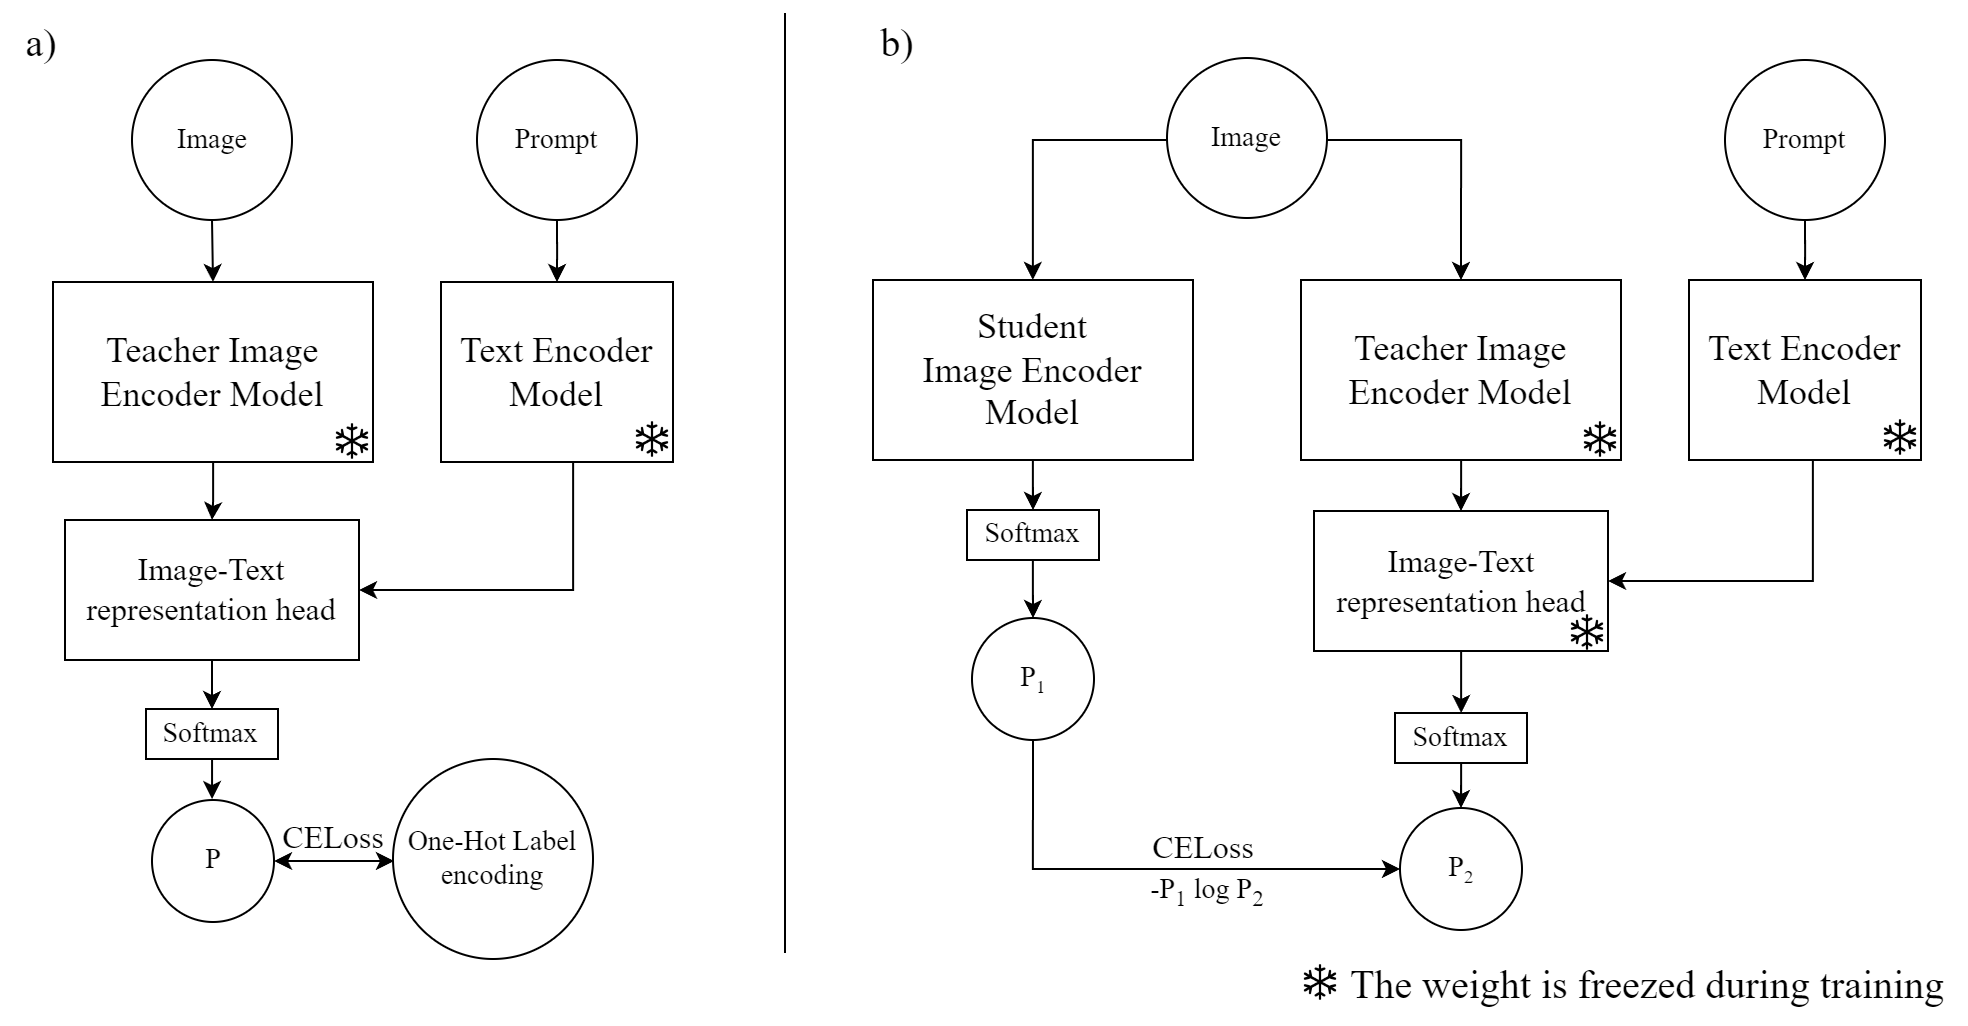
\includegraphics[width=1\textwidth]{Images/Methodology.png}
    \end{center}
    \small a) Training image-text representation head using cross entropy loss b) Self-distillation training by freezing all teacher model
\end{figure}

\begin{figure}[h]
    \caption{Image-Text Cross Attention Classification head}
    \label{fig:cross_attention}
    \centering
    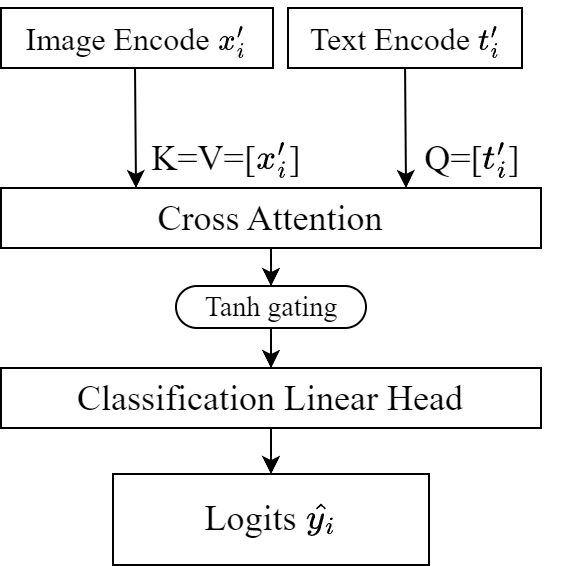
\includegraphics[width=0.5\textwidth]{Images/CrossAttention.png}
\end{figure}

\section{Image-Text Representation Head Training}
\textcolor{red}{todo:change method image to use sub figure a and b}
In the first step as shown in Figure~\ref{fig:methodology}a), the image-text representation head is trained with image-text pairs $(x_i, t_i)$, where $x_i$ is an image input and $t_i$ is a text created with a propmt ``This is an image of [Class]''.
The teacher image encoder $\theta_i$ and the text encoder $\theta_t$ in the training are pre-trained and freezed.
The image and text encoding are obtained by a mapping function $x'_i = f(x_i; \theta_i)$ and $t'_i = f(t_i; \theta_i)$ repectively. 
The image-text representation head as shown in Figure~\ref{fig:cross_attention} which based on an cross-attention and linear classification layer, is produce logits output as Eq.\ref{eq:cross-attention}.
Then, the logits output from the image-text representation head transform into probability distribution output with a softmax function.

\begin{equation} 
    \label{eq:cross-attention}
    \hat{y}_i = Softmax(Attention(K=x'_i, Q=t'_i, V=x'_i))
\end{equation}

The loss function for training the image-text representation head is a cross-entropy as Eq.\ref{eq:loss-cross-attention}, where $y$ is a one-hot label.

\begin{equation}
    \label{eq:loss-cross-attention}
    \mathcal{L}_{Cls} = -y\log\hat{y}
\end{equation}



\section{Self-Distillation}
After training the image-text representation head has trained, the image-text representation head is freezed during the self-distillation process.
The student model have the the same architecture as the teacher image encoder model.
The target for training self-distillation is the softmax output from image-text representation head with the cross entropy loss as a loss function.


% \subsection{Teacher student}
% For the teacher model, we will use two stream encoder based model same as CLIP model \shortcite{dosovitskiy2021an}.
% In this experiment, the teacher vision encoder model will be ResNet \shortcite{he2016deep} and ViT \shortcite{dosovitskiy2021an} version.
% For the student model we used the same architecture as teacher vision encoder model, which are ResNet and ViT.
% \textcolor{red}{todo: Add table describes both image and text encoders.}

% \section{Training Objectives}
% In the first step, we trained the image-text representation head with benchmark datasets by using Cross Entropy loss as describe in \ref{fig:overall_method} a). The image and text encoder was freezed during the first step training. For text input, we used "This is the image of [Class]" as a prompt \shortcite{radford2021learning}. After the first image-text representation head were trained, we create a new student model which have the same architecture as a image encoder model with a linear classification head. The student model was randomly initialized parameters. The objective for self-distillation with teacher and student is

\section{Evaluation}
In this work, the evaulation metric is accuracy evaluated on ImageNet, CIFAR-10 and CIFAR-100.
The student model is evaluated compare to the teacher image encoder model using linear probing and student model trained with self-disillation using single image encoder as a teacher model.

\section{Ablation Study}
- Repeatation self-distillation
- 


